\section{Evaluation}
\label{sec:evaluation}

\subsection{Setup and Metrics}
We evaluate all configurations recorded in \texttt{active\_tile\_pixel\_dataset\_sweep/grid\_search.csv}. The sweep contains 125 settings, with
$\texttt{tile\_width} \in \{14,15,16,17,18\}$,
$\texttt{tile\_height} \in \{14,15,16,17,18\}$, and
$\texttt{min\_active\_pixels} \in \{1,2,3,4,5\}$.
Each configuration is evaluated on 50{,}000 images (\texttt{num\_images=50000}).

We report three groups of metrics:
(1) runtime (\texttt{sparse\_ms}, \texttt{dense\_masked\_ms}, \texttt{dense\_unmasked\_ms}),
(2) tile activity (\texttt{active\_tiles}, \texttt{active\_ratio}), and
(3) recognition quality (Top-1 accuracy fields in the CSV files).
Coverage efficiency is computed from \texttt{config\_tile\_summary.csv} as the fraction of useful ROI pixels among pixels processed inside active tiles.

\subsection{Overall Results}
Across all 125 configurations, sparse latency ranges from \textbf{6.90 ms} to \textbf{14.16 ms} (mean \textbf{8.99 ms}).
By comparison, dense masked latency is 2.15--4.07 ms (mean 2.65 ms), and dense unmasked latency is 1.42--2.87 ms (mean 1.81 ms).
On average, the current sparse implementation is therefore \textbf{3.39$\times$ slower} than dense masked and \textbf{4.97$\times$ slower} than dense unmasked inference.

Top-1 accuracy for sparse inference is very stable: 43.23\%--43.376\% (mean 43.330\%, std 0.026).
Dense masked Top-1 is essentially constant at 43.342\%, while dense unmasked Top-1 stays at 66.82\%.
This indicates that, in the current pipeline, most accuracy loss comes from masking/ROI selection rather than tile threshold tuning.

Coverage efficiency varies from 62.88\% to 71.97\% (mean 67.35\%).
The relation between active tile count and sparse runtime is weak (Pearson $r=-0.052$, Spearman $\rho=-0.041$), suggesting runtime is not explained by active tile count alone.

\subsection{Effect of \texttt{min\_active\_pixels}}
Averaging over all tile-width/height pairs:
threshold 1 gives 9.78 ms latency and 66.01\% coverage efficiency;
threshold 4 gives the best average latency (8.15 ms) with 68.00\% coverage;
threshold 5 further improves coverage to 68.46\% but increases latency to 8.69 ms.
Sparse Top-1 accuracy changes only slightly (43.341\% at threshold 1 vs 43.307\% at threshold 5, i.e., 0.034\% absolute drop).

\begin{table}[t]
\centering
\caption{Representative configurations from the full grid search.}
\label{tab:eval-best-configs}
\begin{tabular}{lcccc}
\hline
Config $(w,h,m)$ & Sparse ms & Coverage (\%) & Active tiles & Sparse Top-1 (\%) \\
\hline
Fastest: $(14,14,4)$ & 6.90 & 71.46 & 106.36 & 43.338 \\
Highest coverage: $(14,14,5)$ & 7.28 & 71.97 & 105.51 & 43.362 \\
Worst latency: $(15,18,3)$ & 14.16 & 66.65 & 92.44 & 43.328 \\
\hline
\end{tabular}
\end{table}

The Pareto frontier in (latency, coverage efficiency) is small and dominated by two nearby points:
$(14,14,4)$ and $(14,14,5)$.
The first is the speed-oriented choice, while the second is the coverage-oriented choice.

\subsection{Kernel-Level Profiling and Dense-Tiled Control}
To understand why sparse inference is still slower than dense inference, we ran an additional micro-benchmark
(\texttt{smallest-test.py}) on an NVIDIA GeForce RTX 5070 with CUDA profiling enabled.
The run used 120 images, 4 representative configurations
($(14,14,4)$, $(14,14,5)$, $(16,16,1)$, $(15,18,3)$),
and chunk sizes from 32 to 2048.
Raw logs are stored in \texttt{smallest-test-result.txt}.

We added a control path called \textit{dense-tiled via sparse path}:
it executes the same tile extraction/writeback pipeline as sparse inference, but with all tiles active.
This isolates implementation overhead from sparsity benefit.

\begin{table}[t]
\centering
\caption{Profiler-derived launch counts and timing summary from \texttt{smallest-test.py}.}
\label{tab:kernel-profile-summary}
\begin{tabular}{lccc}
\hline
Metric & Sparse path & Dense-tiled path & Dense unmasked \\
\hline
Captured CUDA events (min--max) & 1245--1416 & 2001--2259 & 279 \\
Captured CUDA events (mean) & 1311 & 2071 & 279 \\
Forward mean ms (all chunks/configs) & 10.27 & 12.67 & 1.87 \\
\hline
\end{tabular}
\end{table}

\begin{table}[t]
\centering
\caption{Chunk-size sweep averages over 4 representative configurations from \texttt{smallest-test-result.txt}.}
\label{tab:chunk-sweep-avg}
\begin{tabular}{rcccccc}
\hline
\texttt{chunk\_tiles} & Sparse ms & Dense-tiled ms & Dense-unmasked ms & Sparse/Dense-tiled & Dense-tiled/Dense & Sparse/Dense \\
\hline
32   & 15.322 & 13.988 & 1.905 & 1.051 & 7.353 & 7.752 \\
64   & 12.677 & 13.266 & 2.026 & 0.963 & 6.782 & 6.627 \\
128  & 8.954  & 12.194 & 1.870 & 0.735 & 6.582 & 4.833 \\
256  & 9.316  & 12.886 & 1.883 & 0.716 & 6.994 & 4.979 \\
512  & 8.685  & 12.124 & 1.803 & 0.721 & 6.654 & 4.790 \\
1024 & 9.132  & 12.813 & 1.935 & 0.708 & 6.760 & 4.777 \\
2048 & 7.784  & 11.416 & 1.685 & 0.687 & 6.936 & 4.733 \\
\hline
\end{tabular}
\end{table}

\begin{table}[t]
\centering
\scriptsize
\caption{Detailed forward-mean measurements for all tested chunk/config combinations (from \texttt{smallest-test-result.txt}).}
\label{tab:chunk-sweep-detailed}
\resizebox{\linewidth}{!}{
\begin{tabular}{rrrrrrrrrr}
\hline
\texttt{chunk\_tiles} & $w$ & $h$ & $m$ & Sparse ms & Dense-tiled ms & Dense-unmasked ms & Sparse/Dense-tiled & Dense-tiled/Dense & Sparse/Dense \\
\hline
32 & 14 & 14 & 4 & 20.666 & 17.352 & 2.645 & 1.191 & 6.561 & 7.814 \\
32 & 14 & 14 & 5 & 5.630 & 7.448 & 1.090 & 0.756 & 6.834 & 5.165 \\
32 & 15 & 18 & 3 & 17.218 & 16.476 & 1.998 & 1.045 & 8.248 & 8.620 \\
32 & 16 & 16 & 1 & 17.776 & 14.676 & 1.889 & 1.211 & 7.769 & 9.409 \\
64 & 14 & 14 & 4 & 13.844 & 10.983 & 1.415 & 1.260 & 7.760 & 9.782 \\
64 & 14 & 14 & 5 & 11.214 & 14.403 & 2.579 & 0.779 & 5.585 & 4.349 \\
64 & 15 & 18 & 3 & 8.954 & 11.147 & 1.495 & 0.803 & 7.456 & 5.989 \\
64 & 16 & 16 & 1 & 16.694 & 16.532 & 2.613 & 1.010 & 6.327 & 6.389 \\
128 & 14 & 14 & 4 & 9.140 & 12.535 & 2.000 & 0.729 & 6.267 & 4.570 \\
128 & 14 & 14 & 5 & 10.115 & 14.024 & 2.211 & 0.721 & 6.342 & 4.574 \\
128 & 15 & 18 & 3 & 7.823 & 10.853 & 1.456 & 0.721 & 7.452 & 5.372 \\
128 & 16 & 16 & 1 & 8.737 & 11.363 & 1.814 & 0.769 & 6.265 & 4.817 \\
256 & 14 & 14 & 4 & 7.435 & 9.931 & 1.573 & 0.749 & 6.313 & 4.727 \\
256 & 14 & 14 & 5 & 6.484 & 9.679 & 1.326 & 0.670 & 7.297 & 4.888 \\
256 & 15 & 18 & 3 & 8.191 & 11.990 & 1.500 & 0.683 & 7.996 & 5.463 \\
256 & 16 & 16 & 1 & 15.154 & 19.945 & 3.132 & 0.760 & 6.369 & 4.839 \\
512 & 14 & 14 & 4 & 6.864 & 8.812 & 1.396 & 0.779 & 6.315 & 4.918 \\
512 & 14 & 14 & 5 & 7.002 & 10.498 & 1.605 & 0.667 & 6.540 & 4.362 \\
512 & 15 & 18 & 3 & 12.051 & 17.276 & 2.388 & 0.698 & 7.236 & 5.047 \\
512 & 16 & 16 & 1 & 8.825 & 11.910 & 1.825 & 0.741 & 6.525 & 4.835 \\
1024 & 14 & 14 & 4 & 5.455 & 7.885 & 1.121 & 0.692 & 7.035 & 4.867 \\
1024 & 14 & 14 & 5 & 6.345 & 8.699 & 1.391 & 0.729 & 6.253 & 4.561 \\
1024 & 15 & 18 & 3 & 8.038 & 11.776 & 1.573 & 0.683 & 7.487 & 5.111 \\
1024 & 16 & 16 & 1 & 16.690 & 22.892 & 3.654 & 0.729 & 6.266 & 4.568 \\
2048 & 14 & 14 & 4 & 11.255 & 16.278 & 2.712 & 0.691 & 6.002 & 4.150 \\
2048 & 14 & 14 & 5 & 5.852 & 8.387 & 1.288 & 0.698 & 6.513 & 4.544 \\
2048 & 15 & 18 & 3 & 7.460 & 12.267 & 1.454 & 0.608 & 8.436 & 5.130 \\
2048 & 16 & 16 & 1 & 6.570 & 8.733 & 1.286 & 0.752 & 6.792 & 5.109 \\
\hline
\end{tabular}
}
\end{table}

Key observations are:
(1) launch volume is much higher on tiled paths than on dense unmasked inference;
(2) sparse is generally faster than dense-tiled once chunk size is large enough (indicating real pruning benefit inside the same execution path);
but
(3) both tiled paths remain far slower than the dense unmasked path.
Across all runs, dense-tiled is on average 6.87$\times$ slower than dense unmasked (range 5.59$\times$--8.44$\times$).
This indicates that the dominant bottleneck is tiled execution overhead (many small kernels and tensor movement), not just arithmetic count.

Chunk size tuning helps but does not close the gap.
Averaged over the 4 benchmarked configurations, sparse forward time drops from 15.32 ms at \texttt{chunk\_tiles=32}
to 7.78 ms at \texttt{chunk\_tiles=2048} (about 1.97$\times$ speedup),
yet remains substantially above dense unmasked (1.69 ms at \texttt{chunk\_tiles=2048} benchmark block).

Profiler kernel names further support this interpretation:
the sparse/tiled paths are dominated by repeated elementwise copy/fill kernels and batched copy/scatter-style kernels
(\texttt{direct\_copy\_kernel\_cuda}, \texttt{FillFunctor}, \texttt{CatArrayBatchedCopy}, clamp/mul elementwise ops),
whereas dense unmasked inference uses a much smaller launch set dominated by optimized convolution/Bn kernels.

\subsection{Visual Analysis}
Figure~\ref{fig:grid-overview} summarizes the full parameter sweep.
Figure~\ref{fig:coverage-scatter} and Figure~\ref{fig:runtime-scatter} show that higher coverage can often be achieved without large accuracy changes, while runtime behavior is more irregular than a simple linear function of active tile count.

\begin{figure}[t]
\centering
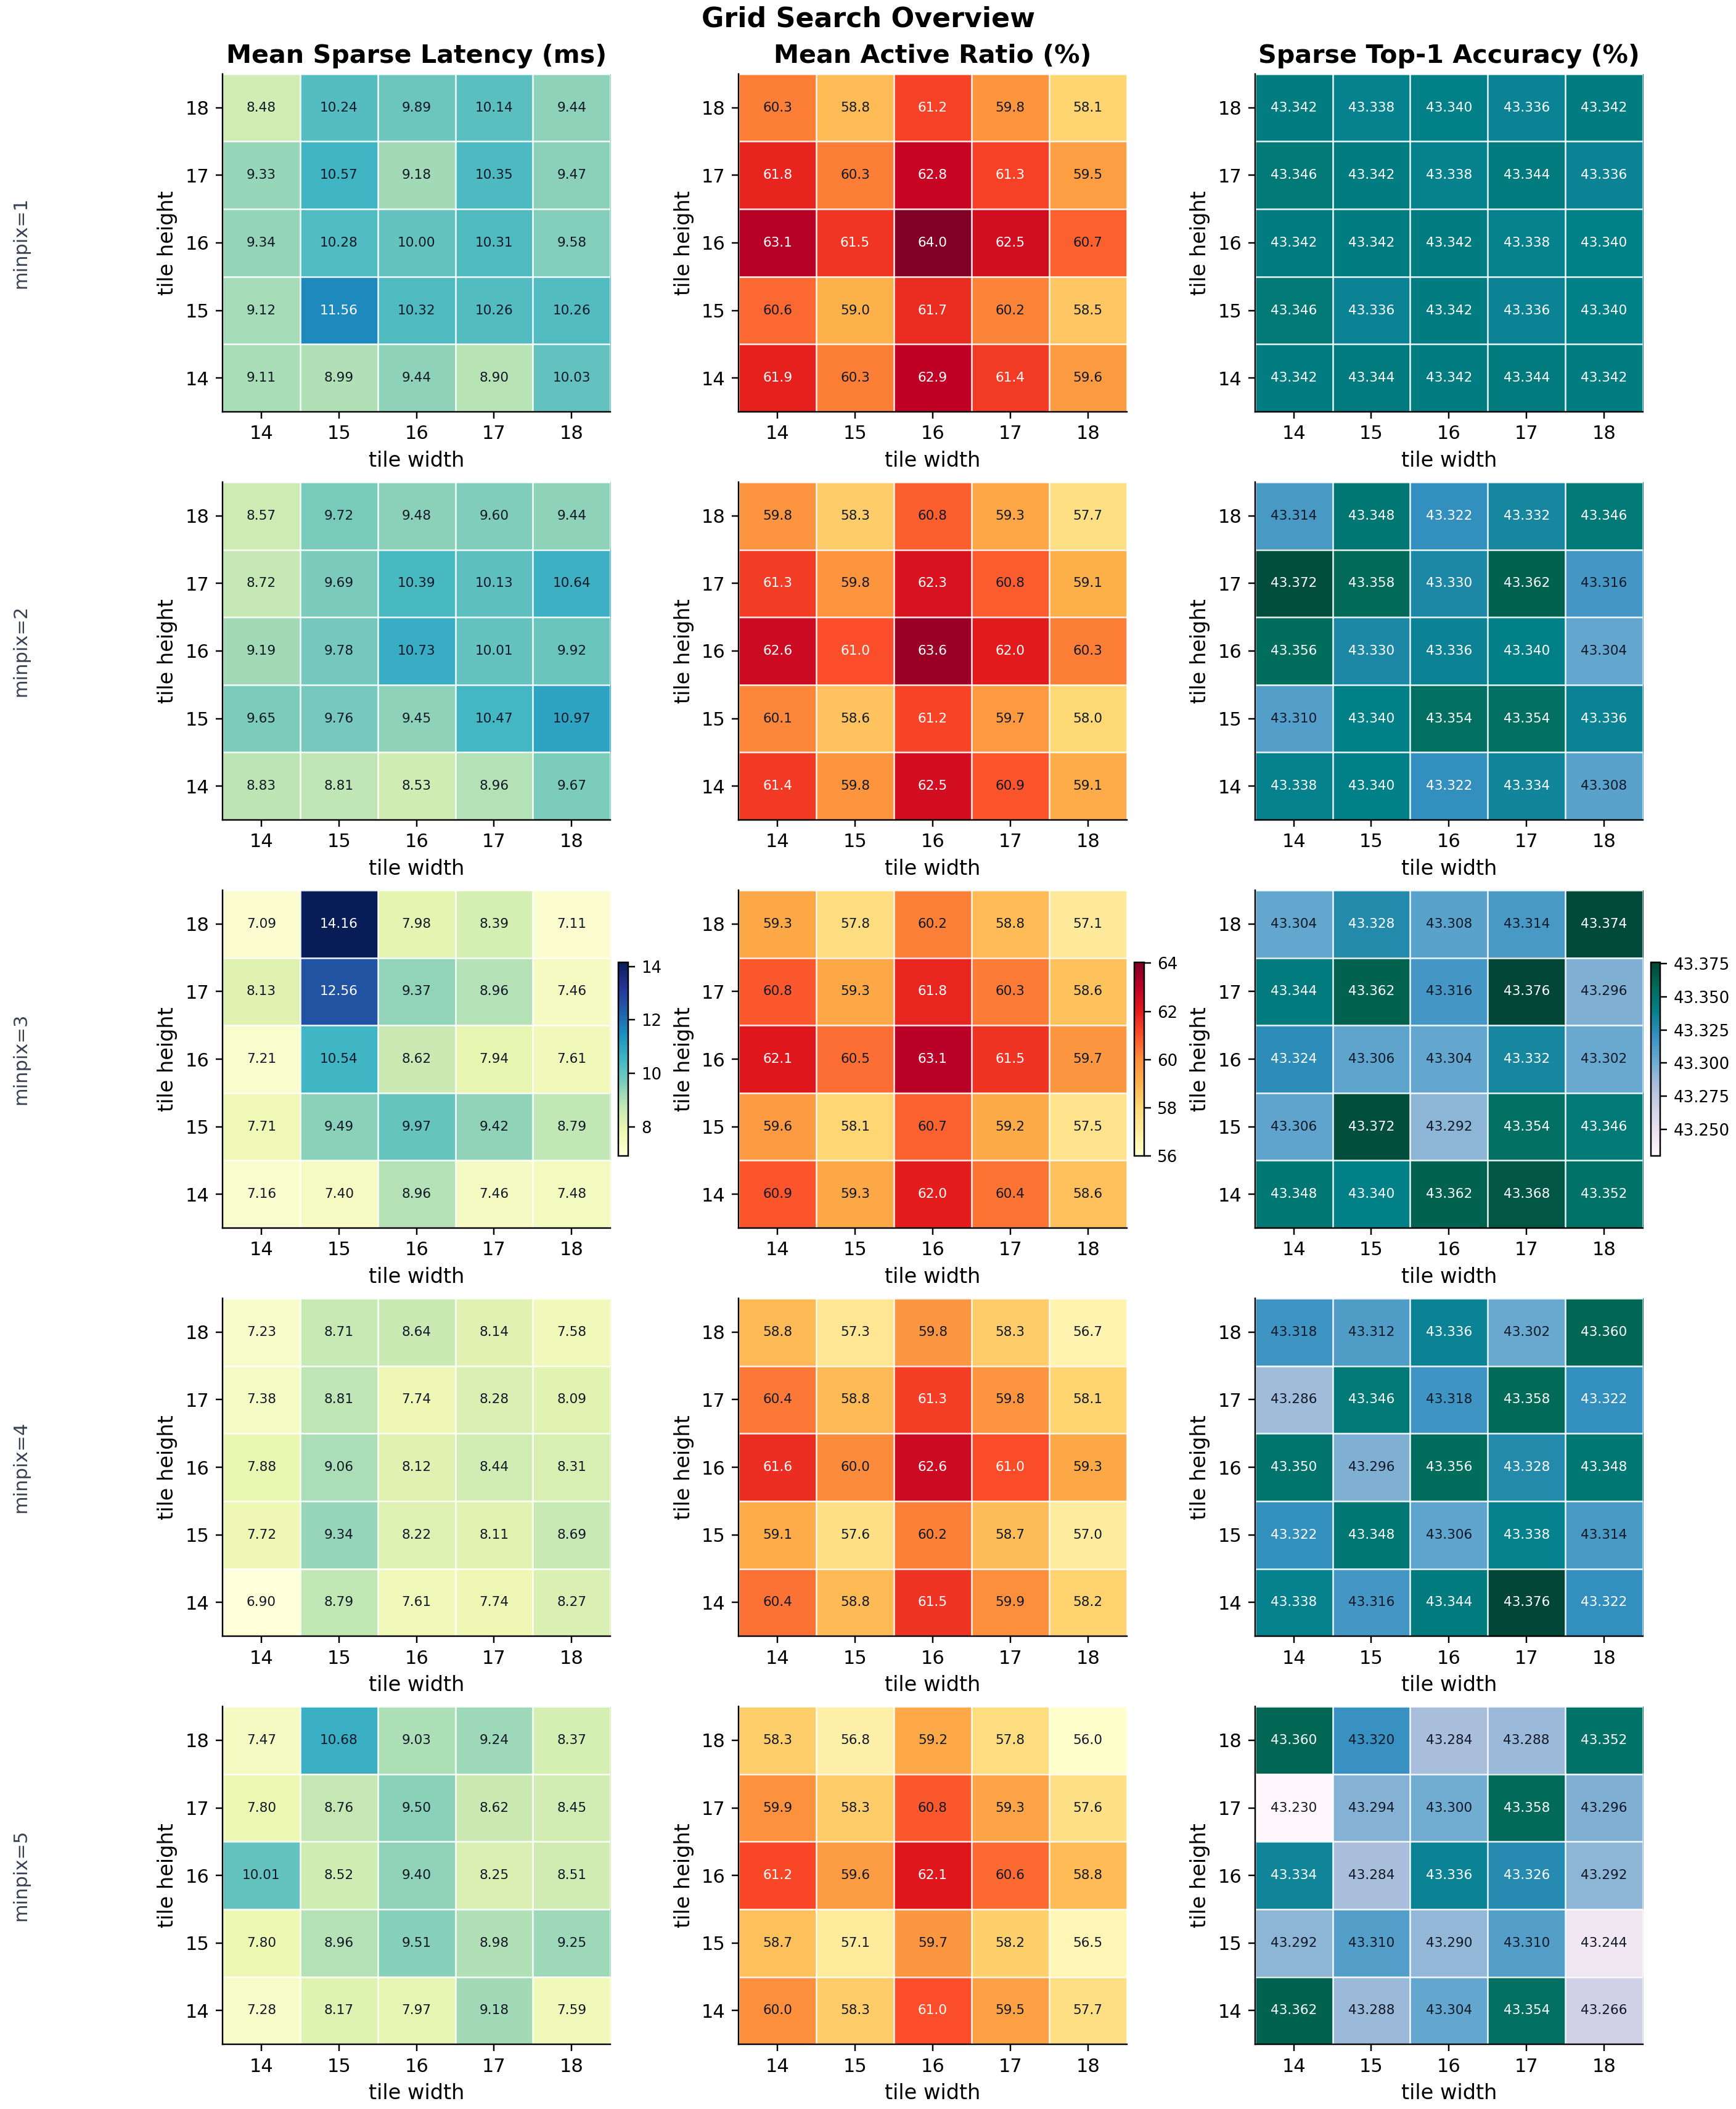
\includegraphics[width=\linewidth]{active_tile_pixel_dataset_sweep/grid_search_overview.png}
\caption{Grid-search heatmaps for sparse latency, active ratio, and sparse Top-1 accuracy.}
\label{fig:grid-overview}
\end{figure}

\begin{figure}[t]
\centering
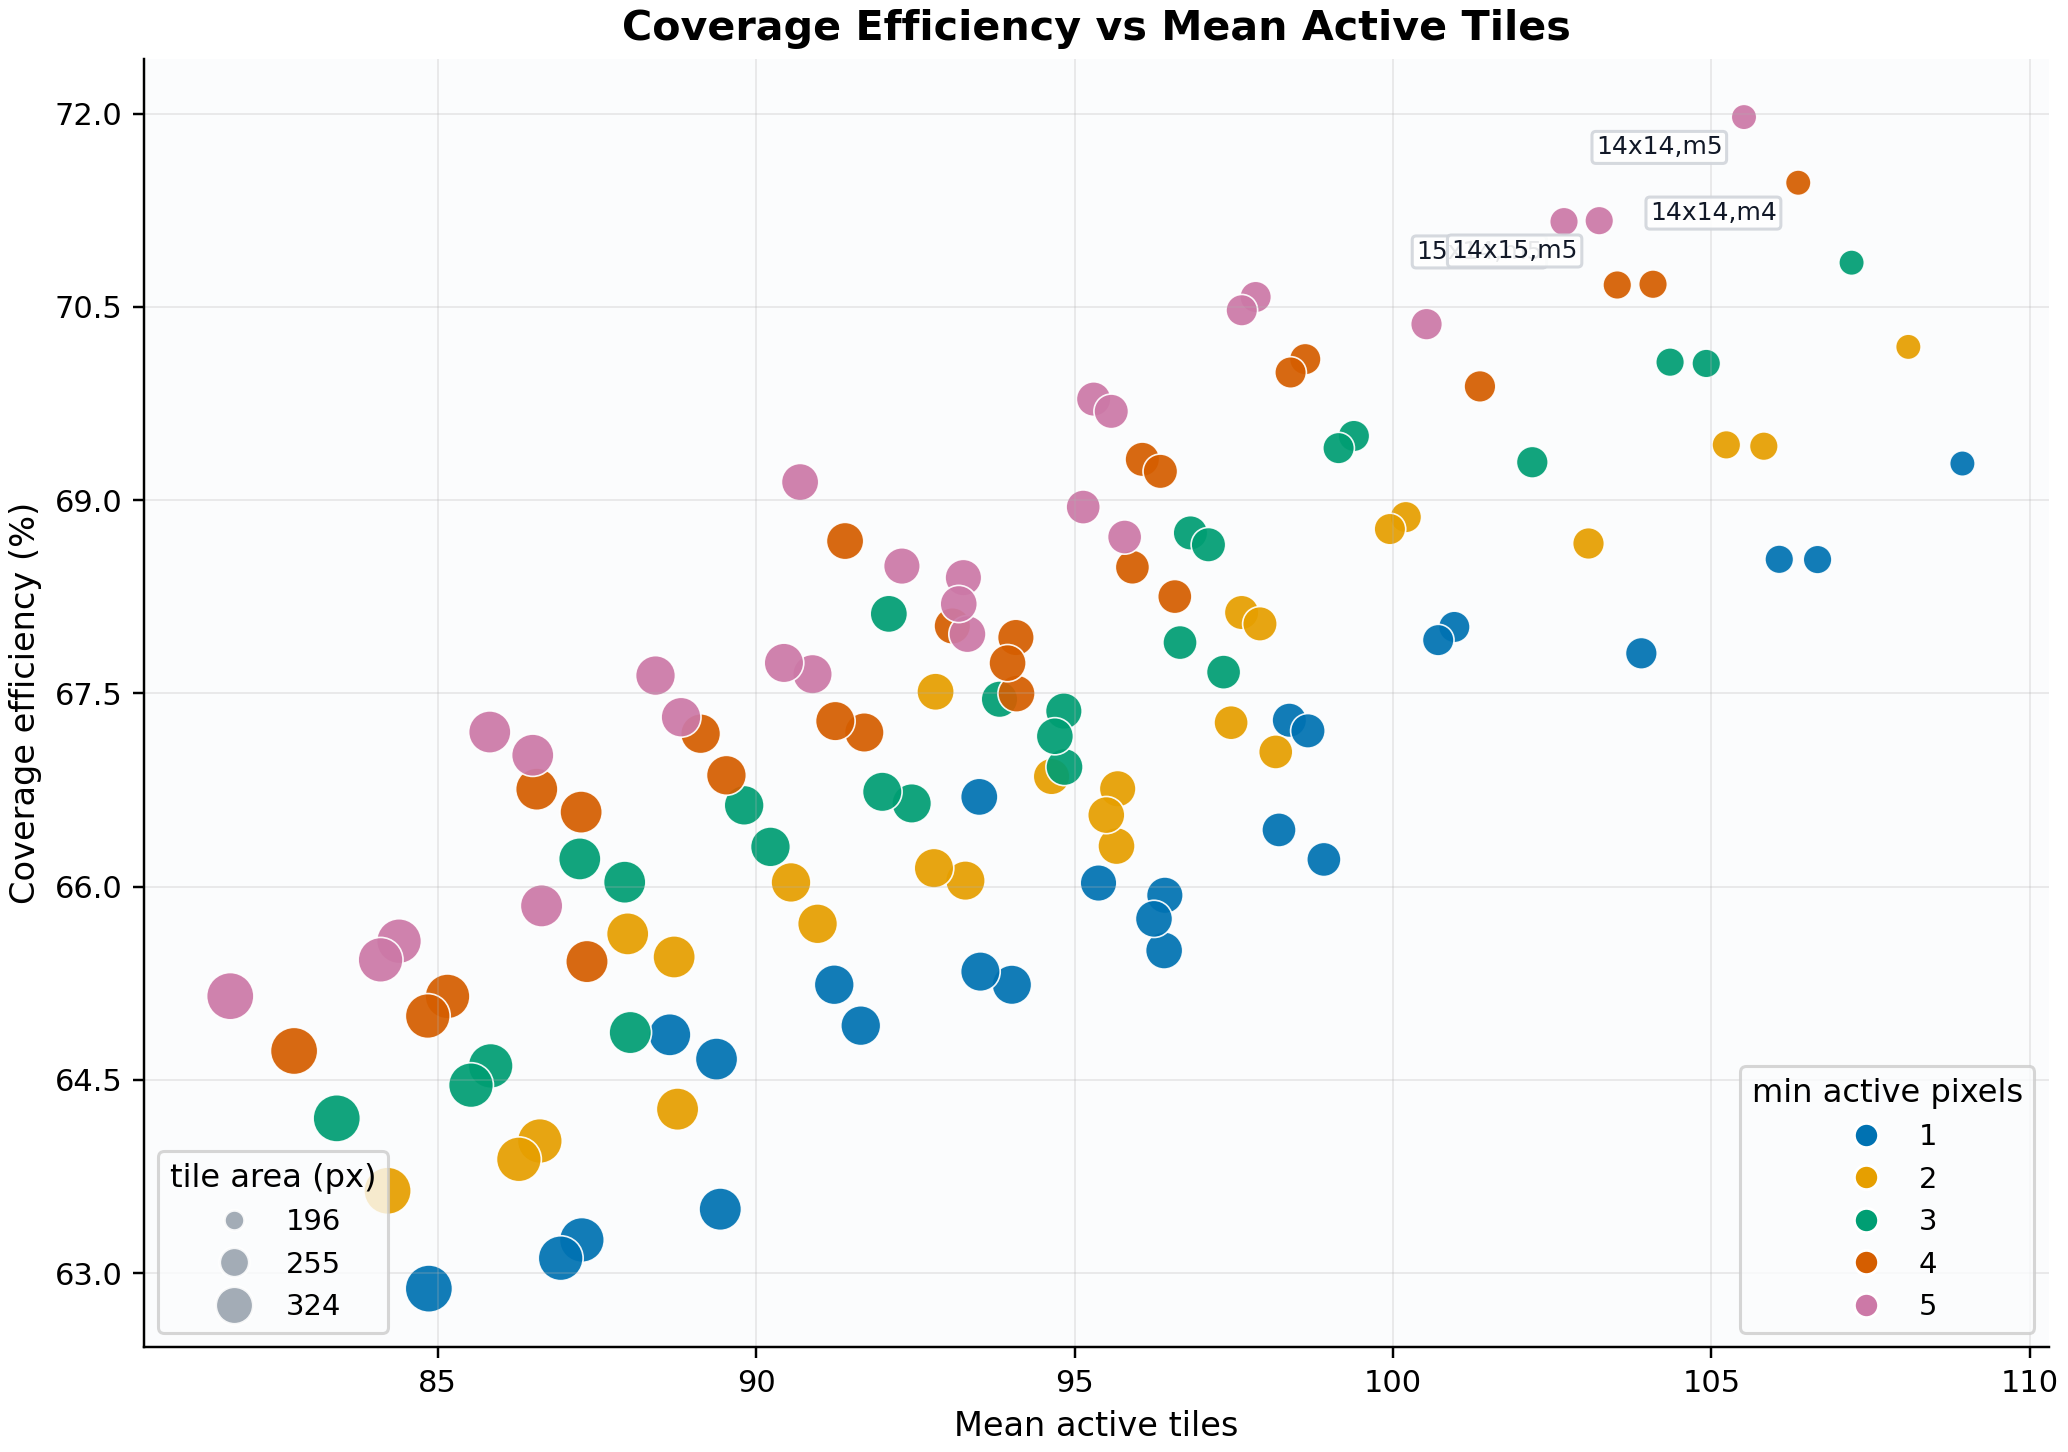
\includegraphics[width=0.92\linewidth]{active_tile_pixel_dataset_sweep/coverage_efficiency_by_config.png}
\caption{Coverage efficiency versus mean active tiles across all configurations.}
\label{fig:coverage-scatter}
\end{figure}

\begin{figure}[t]
\centering
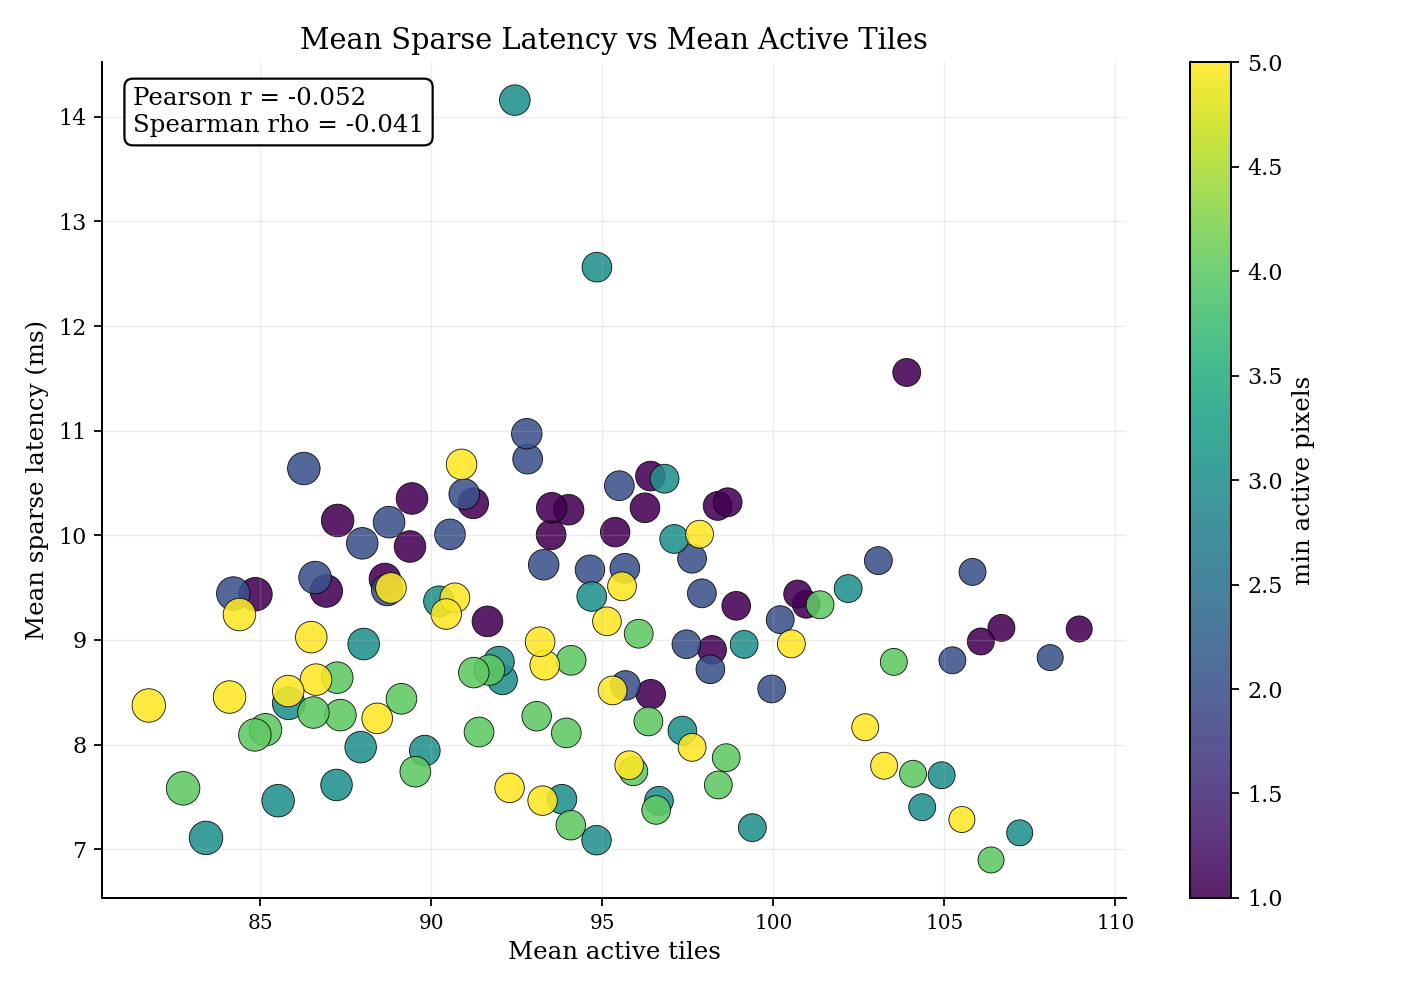
\includegraphics[width=0.92\linewidth]{active_tile_pixel_dataset_sweep/runtime_vs_active_tiles.png}
\caption{Sparse runtime versus mean active tiles with correlation statistics and trend line.}
\label{fig:runtime-scatter}
\end{figure}
